%%%%%%%%%%%%%%%%%%%%%                                                                           
% SHAPE RECOGNITION
% TEMA 2
%%%%%%%%%%%%%%%%%%%%%
  
\documentclass[12pt]{article}
  
\usepackage[T1]{fontenc}
\usepackage{indentfirst}
\usepackage{graphicx}
\usepackage{titling}
\usepackage{float}
\usepackage{subfig}
\usepackage{wrapfig}
\usepackage{gensymb}
\usepackage{amsmath}
\usepackage{listings}
\usepackage{matlab-prettifier}
\usepackage{hyperref}
\usepackage{float}
  
  
\begin{document}

\begin{titlepage}
    \begin{center}
        \vspace*{1cm}

        \Huge
        \textbf{Recunoașterea formelor}

        \vspace{0.5cm}
        \LARGE
        Tema 2

        \vspace{1.5cm}

        \textbf{Sebastian Lăzărescu}

        \vfill

        \Large
        Facultatea de Automatică și Calculatoare\\
        Universitatea Tehnică „Gheorghe Asachi” din Iași\\
        Mai 2025
    \end{center}
\end{titlepage}

\section{Rezultate}

\begin{figure}[H]
    \centering
    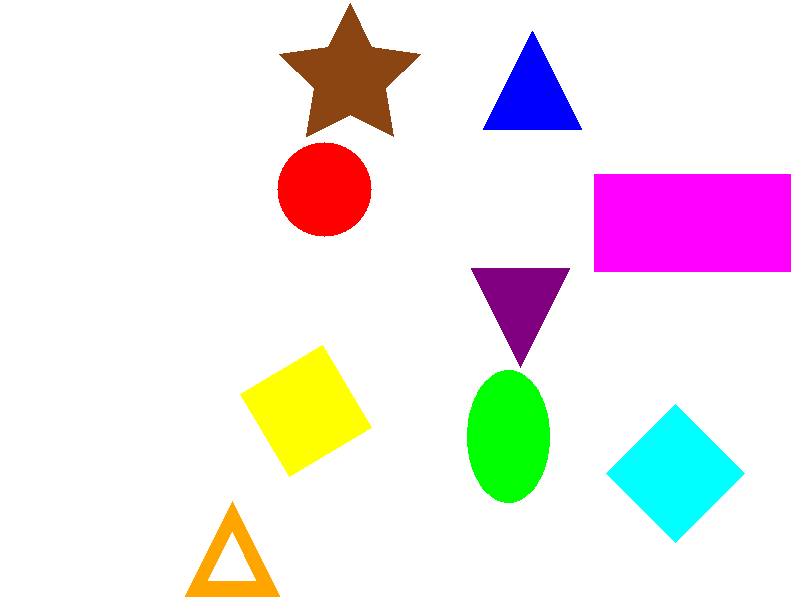
\includegraphics[width=0.7\textwidth]{../images/shapes.png}
    \caption{Imaginea pentru testarea algoritmului}
\end{figure}

\begin{figure}[H]
    \centering
    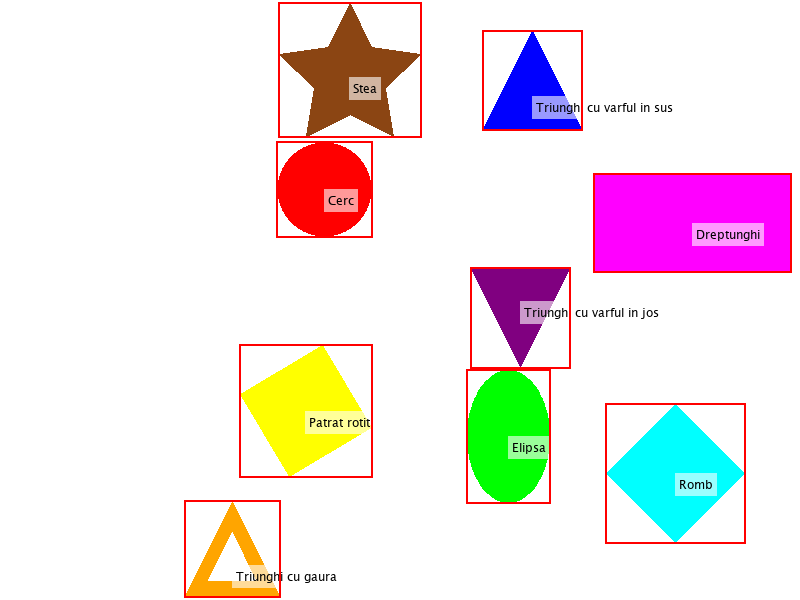
\includegraphics[width=0.7\textwidth]{../images/final_image.png}
    \caption{Imaginea finală}
\end{figure}

\section{Pasul 1: Preprocesare imagine}


La aceast pas, imaginea de intrare este prelucrată pentru a fi adusă 
într-o formă adecvată procesării ulterioare. Etapele sînt următoarele: \\

\textbf{Etapa 1: \emph{Conversia în tonuri de gri}}. Aici s-a folosit funcția
MATLAB \emph{rgb2gray}. \\

\textbf{Etapa 2: \emph{Binarizarea imaginii}}. Se aplică binarizarea imaginii în 
tonuri de gri folosind un prag fix (\emph{T = 0.89}). \\

\textbf{Etapa 3: \emph{Operații morfologice}}. Se definește un element structurant 
pătrat de 5x5 pixeli. Se aplică operația morfologică de deschidere (\emph{imopen}), care
elimină zgomotul de mici dimensiuni și separă obiectele apropiate. Imaginea
rezultată este apoi inversată (\~{}) \\

\textbf{Etapa 4: \emph{Etichetarea obiectelor}}. Obiectele conectate din imaginea
binară curățată sînt etichetate folosind conectivitatea de 4 pixeli. Fiecărui 
obiect i se atribuie o etichetă unică. Imaginea etichetată este apoi convertită 
într-o imagine color cu funcția \emph{label2rgb}, pentru o vizualizare mai ușoară a 
obiectelor identificate. \\

\section{Pasul 2: Detectarea formelor}

Pentru detecția formelor m-am folosit de proprietățile fiecărui obiect detectat.
Proprietățile au fost "achiziționate" cu ajutorul funcției MATLAB \emph{regionprops}. \\

\textbf{Detecția triunghiurilor:} \\
\indent Din analiza proprietăților se observă că triunghiurile au proprietatea \emph{Eccentricity}
aproximativ \emph{0.5000}, deci verificăm ca această proprietate să fie cuprinsă între 
\emph{0.4890} și \emph{0.5050}. 

Pentru a detecta un triunghi cu gaură, ne folosim de
proprietatea \emph{EulerNumber}. Dacă aceasta este 0, rezultă că obiectul respectiv are
o gaură în el.

Pentru a vedea dacă triunghiul este cu vîrful în sus sau în jos, am scos toți pixelii
de pe obiectul detectat, am făcut 2 benzi (banda de sus și banda de jos) cu pixelii cei
mai de sus și cei mai de jos, am calculat lungimea acestor benzi și am verificat care este
mai mare. Dacă banda de sus < banda de jos, rezultă triunghi cu vîrful în sus, iar dacă
banda de sus > banda de jos, rezultă triunghi cu vîrful în jos. \\

\textbf{Detecția cercurilor și a elipselor:} \\
\indent Pentru detectarea cercurilor și a elipselor, m-am folosit de proprietatea
\emph{Circularity}. Aceasta arată cît de "cerc" este un obiect. Dacă \emph{Circularity} 
> \emph{0.9}, sînt șanse foarte mari ca obiectul să fie cerc sau elipsă. Pentru a 
face distincția dintre cerc și elipsă, m-am folosit de \emph{Eccentricity}. Dacă este 0,
înseamnă că obiectul este sută la sută cerc. Dacă este diferit de 0, rezultă că este elipsă
(în cazul nostru). \emph{Eccentricity} ne spune cît de alungit este un cerc. \\

\textbf{Detecția pătratelor, pătratelor rotite și a romburilor:} \\
\indent Verificăm ca \emph{MajorAxis} și \emph{MinorAxis} să fie egale și \emph{Circularity} <
\emph{0.9} (și cercurile au axele egale). Dacă avem \emph{Orientation} diferit de 0, rezultă
că figura este rotită. Dacă \emph{Extent} (care arată cît din figură este încadrată în BoundingBox)
este 1, rezultă pătrat, iar dacă \emph{Extent} este 0.5, rezultă că avem un romb. \\

\textbf{Detecția dreptunghiurilor:} \\
\indent Dacă \emph{Extent} este 1 (adică sută la sută încadrat în BoundingBox) și axele nu sînt
egale și emph{Solidity} este 1, rezultă că avem un dreptunghi. \emph{Solidity} ne spune
cît de "plină" este o figură în comparaițe cu \emph{convex hull}. \\

\textbf{Detecția stelelor:} \\
\indent Pentru a detecta stelele, m-am folosit de \emph{Solidity}. Steaua are foarte multe coțuri
deci nu "umple" foarte mult.
\end{document}
